\section{Installation et connexion d'Apache Griffin \`a PostgreSQL}
\subsection{Installation de l'outil}
Apache Griffin, offre l'avantage d'avoir une documentation bien r\'edig\'ee et plut\^ot d\'etaill\'ee, disponible sur \href{https://github.com/apache/griffin}{github}. Pour son installation, deux modes sont propos\'es : 
\begin{itemize}[parsep=0cm,itemsep=0cm]
\item une installation en utilisant des conteneurs docker ou;
\item une installation \`a partir de z\'ero  des diff\'erentes applications de son \'ecosyst\`eme.
\end{itemize}
Le deuxi\`eme mode est privil\'egi\'e lorsqu'on souhaite configurer les composantes de Griffin et dimensionner l'architecture suivant des exigences particuli\`eres. Tandis que, l'installation via docker est recommand\'ee si on n'envisage que de tester les fonctionnalit\'es de  Griffin; ce qui est notre cas ici pr\'esent. Pour chacun de ces modes, un processus diff\'erent est propos\'e  suivant qu'on souhaite analyser des donn\'ees en \textit{streaming} ou en \textit{batch}. L'objectif vis\'e dans un premier temps en installant Apache Griffin, est de r\'eussir \`a le connecter \`a PostgreSQL. Nous avons donc opt\'e pour une installation de type \textit{batch}. Ce choix est motiv\'e par le fait que l'audit de la qualit\'e des donn\'ees se fera de façon p\'eriodique sur des extractions.
\\

Pour l'installation et la r\'ealisation des tests , nous avons utilis\'e notre propre ordinateur portable. Il s'agit d'un ordinateur portable ayant les caract\'eristiques suivantes: 
\begin{itemize}[parsep=0cm,itemsep=0cm]
\item M\'emoire \acrshort{ram} : 16 Gigaoctet;
\item Processeur:  Intel Core i7-8565U \acrshort{cpu} \@ 1.80GHz × 8;
\item M\'emoire disque : 1 T\'eraoctet en \acrshort{hdd} (\acrlong{hdd}) et 300 Gigaoctet en \acrshort{ssd} (\acrlong{ssd});
\item Carte Graphique d\'edi\'ee : NVIDIA Corporation GP107M [GeForce GTX 1050 Mobile];
\item Syst\`eme d'exploitation : Ubuntu 20.04.3 \acrshort{lts} 64-bit install\'e en dual-boot.
\end{itemize}

L'installation via docker se d\'eroule en deux principales \'etapes, conform\'ement \`a la documentation \cite{ApacheGriffinDocDocker}. Dans un premier temps, une pr\'eparation de l'environnement de travail est requise. Cette \'etape est r\'ealis\'ee en trois (3) points essentiels: 
\begin{enumerate}[parsep=0cm,itemsep=0cm]
\item l'installation de docker et docker compose;
\item l'augmentation des limites de la m\'emoire virtuelle en vue de l'utilisation d'Elasticsearch;
\item la r\'ecup\'eration des images docker n\'ecessaires pour l'installation.
\end{enumerate}
\vspace{0.15cm}

Docker est une plateforme de conteneurisation, qui permet la création et l'utilisation de conteneurs Linux. Un conteneur est comme une machine virtuelle très légère et modulaire et est donc une tr\`es bonne alternative \`a ces derni\`eres. En outre, les conteneurs offrent une grande flexibilité : on peut les créer, déployer, copier et déplacer d'un environnement à un autre, ce qui permet d'optimiser les applications pour le cloud \cite{RedHatDocker}. Un conteneur docker est une instance exécutable d’une image docker. Une image quant \`a elle est un fichier immuable, qui constitue essentiellement une capture instantanée d’un conteneur \cite{WayToLearnX_docker}. Il s’agit d’un ensemble de processus logiciels légers et indépendants, regroupant tous les fichiers nécessaires à l’exécution des processus : codes, \textit{runtime}, outils systèmes, bibliothèques et paramètres. Docker Compose ou Compose est quant \`a lui un outil de docker qui permet de d\'efinir et d'ex\'ecuter des applications multi-conteneurs \cite{Dockerdoc}. Gr\^ace aux configurations \'ecrites dans un fichier \acrshort{yaml} (\acrlong{yaml}), il permet de cr\'eer un ensemble de services (conteneurs, r\'eseaux, volumes), de les d\'emarrer et de les arr\^eter tous en m\^eme temps.
\\

Les images docker n\'ecessaires pour le bon fonctionnement de Griffin en mode \textit{batch} sont: 
\begin{itemize}[parsep=0cm,itemsep=0cm]
\item \textbf{apachegriffin/griffin\_spark2}:  Cette image contient les logiciels suivants:  MySQL, PostgreSQL, Apache Hadoop, Apache Hive, Apache Spark, Apache Livy ainsi que les modules Service et Measure d'Apache Griffin. De m\^eme, on y trouve \'egalement  quelques données de test. Elle fonctionne comme un \textit{cluster} Spark à un seul nœud, fournissant le moteur Spark et le service Apache Griffin.
\item \textbf{apachegriffin/elasticsearch}: Cette image est une surcouche de l'image officielle de la version 4 d'Elasticsearch. Elle a \'et\'e configur\'ee pour permettre la r\'eception de requêtes \acrshort{cors} (\acrlong{cors}: partage de ressources entre origines multiples) ainsi que la sauvegarde des métriques.
\end{itemize}
%\vspace{0.15cm}

En plus de ces images, nous avons utilis\'e :
\begin{itemize}[parsep=0cm,itemsep=0cm]
\item \textbf{postgres}:  Il s'agit l\`a, de la derni\`ere version de l'image de PostgreSQL. Elle servira pour les tests de connexion.
\item \textbf{docker.elastic.co/elasticsearch/elasticsearch:7.13.1}: Cette image est utilis\'ee en lieu et place de l'image apachegriffin/elasticsearch. Ce changement a \'et\'e fait pour faciliter l'utilisation de Kibana pour la visualisation.
\item \textbf{docker.elastic.co/kibana/kibana:7.13.1}: Kibana est une plateforme open source d'analyse et de visualisation conçue pour fonctionner avec Elasticsearch.
\end{itemize}
\vspace{0.15cm}


Apr\`es la pr\'eparation de l'environnement, l'\'etape qui suit est la cr\'eation des diff\'erents conteneurs. \`A cette \'etape, la documentation \cite{ApacheGriffinDocDocker} fournit un fichier \emph{docker-compose-batch.yml}. Ce fichier d\'efinit deux principaux services : \emph{griffin} et \emph{es} (elasticsearch). Ce sont des conteneurs instanci\'es \`a partir des images propos\'ees par la documentation. Le fichier \emph{docker-compose-batch.yml} sp\'ecifie \'egalement le mappage des ports pour chaque conteneur, ainsi que le nom du conteneur, celui de la machine virtuelle et les liens entre les conteneurs. \`A cette \'etape, nous avons d\'efini une nouvelle configuration, afin de mieux organiser notre architecture. En effet, cette configuration tient compte des nouvelles images ajout\'ees. En plus des services pr\'ec\'edemment cit\'es, nous avons ajout\'e un conteneur Kibana configur\'e et li\'e selon les sp\'ecifications de \cite{EsKibana} ainsi qu'un conteneur postgres, tout en prenant soin de substituer l'image d'Elasticsearch par une version plus r\'ecente. Un service r\'eseau a \'et\'e ajout\'e. Il permet la cr\'eation d'un sous r\'eseau de type \textit{bridge}. Cette configuration permet d'attribuer de façon statique des adresses \acrshort{ip} (\acrlong{ip}) aux diff\'erents conteneurs. Un dernier service de stockage persistant avec la machine h\^ote fut \'egalement ajout\'e. Avec un tel stockage, les fichiers de configuration des jobs griffin sont sauvegard\'es, m\^eme en cas de perte ou de suppression des conteneurs.
\\

\begin{figure}[H]
    \caption{Architecture mise en place pour tester Apache Griffin}  \label{fig:xray}
    \begin{center}
      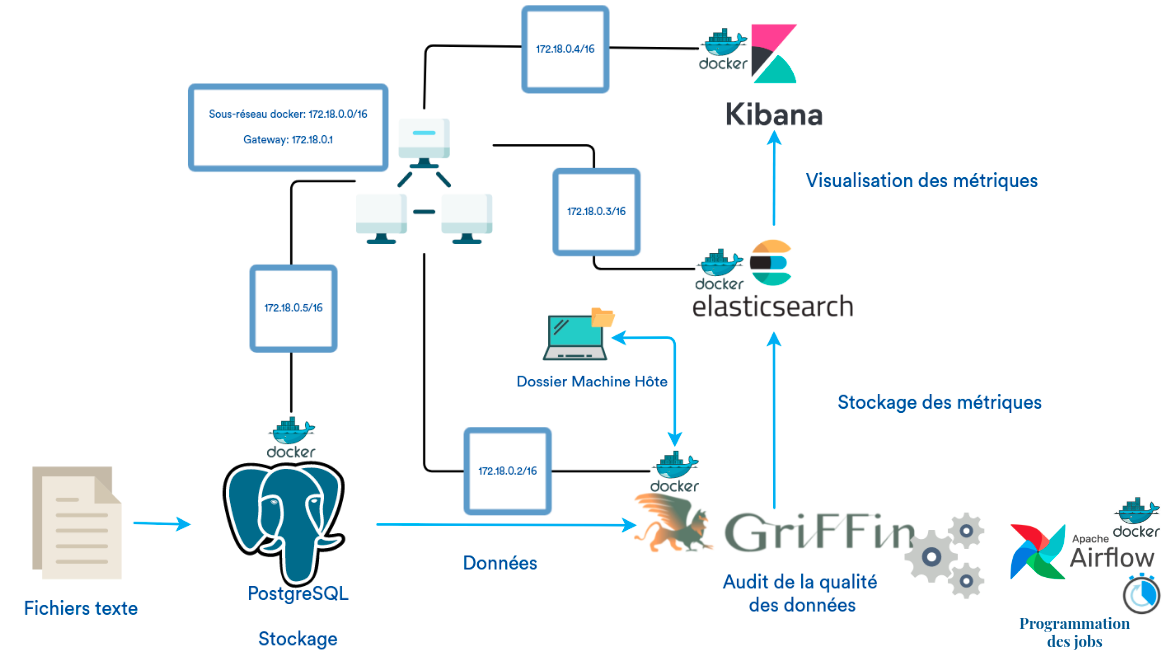
\includegraphics[scale=0.43]{Main/Static/Archi_test_2.png} 
    \end{center}
\end{figure}
Suite \`a l'installation de Griffin, il est alors possible d'utiliser ses diff\'erentes fonctionnalit\'es. On peut  donc avoir acc\`es \`a son interface graphique, ex\'ecuter des requ\^etes par l'entremise de Postman pour la r\'ealisation des t\^aches de qualit\'e de donn\'ees ou simplement l'utiliser en ligne de commande via le conteneur griffin. 

\subsection{Connexion}
L'\'evaluation de la qualit\'e des donn\'ees, n\'ecessite bien \'evidemment des donn\'ees. \`A cet effet, Griffin permet de configurer l'acc\`es \`a diff\'erentes sources de donn\'ees. Notamment, en mode \textit{batch}, Griffin peut auditer la qualit\'e des donn\'ees situ\'ees dans des tables Hive, dans des fichiers AVRO, des fichiers plats (Parquet, \acrshort{csv}, \acrshort{tsv}, \acrshort{orc}) et des donn\'ees provenant de sources poss\'edant des pilotes \acrshort{jdbc} (\acrlong{jdbc}) comme Oracle, MySQL, PostgreSQL... C'est notamment cette derni\`ere facult\'e qui est utilis\'ee pour r\'ealiser la connexion \`a PostgreSQL. Comme \'enonc\'e pr\'ec\'edemment, plusieurs modalit\'es d'acc\`es sont disponibles pour l'utilisation de Griffin. Pour une manipulation plus conviviale, l'interface web est privil\'egi\'ee. Toutefois, elle pr\'esente quelques limites. En effet, actuellement l'interface web ne prend en charge que quelques dimensions (Accuracy, Profiling, Publish Metrics) ainsi que l'acc\`es aux tables Hive. Cette limitation se pr\'esente au niveau du module Service et de ce fait impacte \'egalement l'utilisation de Postman. Par contre, l'utilisation directe en ligne de commande gr\^ace \`a la soumission d'un \textit{job} Spark, est conforme aux fonctionnalit\'es d\'ecrites dans la documentation. Elle rend n\'eanmoins la t\^ache moins ais\'ee. Ce mode de fonctionnement passe directement par le module Measure. Il va s'en dire que c'est par ce moyen que les tests ont \'et\'e effectu\'es.
\\

Dans le vocabulaire de Griffin, une \textbf{mesure} (\textit{measure}) est la mat\'erialisation d'une dimension de  qualit\'e de donn\'ees. Il s'agit de l'\'ecriture de la requ\^ete caract\'erisant les attentes ou sp\'ecificit\'es de la dimension consid\'er\'ee. Elle contient les r\`egles \`a \'evaluer. L'ex\'ecution de cette mesure est appel\'ee un \textbf{\textit{job}} et les informations num\'eriques qui sont produites sont qualifi\'ees de \textbf{m\'etriques}. Ces informations peuvent aussi \^etre des extractions de donn\'ees. L'utilisation en ligne de commande, fait intervenir l'acc\`es au \acrshort{bash} (\acrlong{bash} interpréteur en ligne de commande de type script) du conteneur griffin. Elle requiert \'egalement la configuration manuelle des mesures au moyen d'un fichier d'extension \textit{.json} (\acrfull{json}). Ce fichier contient les informations d\'ecrivant la source de donn\'ees, \'eventuellement les acc\`es (identifiant et mot de passe) ainsi que la ou les r\`egles de qualit\'e des donn\'ees qui seront \'evalu\'ees, comment les \'evaluer et o\`u stocker les r\'esultats. Une description plus d\'etaill\'ee du fichier de configuration est fournie dans la \hyperref[sec:TestGriffin]{section suivante}. Retenons pour l'instant que pour r\'ealiser la connexion \`a une source de type \acrshort{jdbc}, les informations suivantes sont n\'ecessaires:
 \begin{itemize}[parsep=0cm,itemsep=0cm]
 \item \textbf{le type de connexion}: \acrshort{jdbc} ; 
 \item \textbf{la base de donn\'ees}: demo ; 
 \item \textbf{la table cibl\'ee}: test\_auto;
 \item \textbf{l'url de connexion}: jdbc:postgresql://172.18.0.5:5432/demo;
 \item \textbf{le nom d'utilisateur pour la connexion}: aurel;
 \item \textbf{le mot de passe}: 123456789;
 \item \textbf{le pilote JDBC}: org.postgresql.Driver . 
 \end{itemize}
\vspace{0.15cm}

N\'eanmoins, bien que le code source du module Measure ait pr\'evu une \textit{class} gouvernant les sources de type \acrshort{jdbc}, la connexion avec une base de donn\'ees PostgreSQL n'\'etait pas nativement prise en charge. En effet, cela \'etait d\^u \`a l'absence du pilote de connexion dans le \textit{Classpath}\footnote{Chemin d'accès au répertoire où se trouvent les classes et les packages Java \\} du projet. Pour y rem\'edier nous avons donc modifi\'e le code source du module Measure. Cette modification passe par l'ajout aux d\'ependances du projet dans le fichier \emph{Pom.xml}, du pilote de connexion \`a une base de donn\'ees PostgreSQL. Puis au niveau des fichiers de test, il fallait adapter le code, afin qu'\`a la phase de \textit{build} \footnote{Phase de compilation d'un projet conduisant \`a la cr\'eation d'un fichier \textit{.jar} \\} du projet, le pilote une fois t\'el\'echarg\'e soit convenablement ajout\'e au \textit{Classpath}. Cette phase conduit \'egalement \`a la cr\'eation d'un nouveau \textit{.jar} du module Measure. Il est \`a noter que la version de Griffin disponible dans l'image propos\'ee est la 0.2.0 alors que la derni\`ere version officiellement disponible \`a la date de r\'edaction ,est la version 0.6.0. La modification du code source a donc \'et\'e op\'er\'ee sur la version 0.6.0. Une fois la nouvelle version obtenue, nous avons entrepris de construire une nouvelle image de griffin en prenant comme image de base apachegriffin/griffin\_spark2:0.3.0. C'est notamment cette nouvelle image qui est utilis\'ee dans notre fichier docker-compose. Elle est baptis\'ee griffin: 0.6.2 . Et c'est suivant ce processus \cite{ApacheGriffinDocDockerDevEnvBuild}, que nous avons pu avoir une image \`a jour permettant d'interconnecter griffin et PostgreSQL.

\section{Fonctionnalit\'es attendues d'Apache Griffin}
\label{sec:TestGriffin}

%\`A cet effet, une série de \textit{tokens} de qualit\'e des donn\'ees a \'et\'e \'emise pour tester les fonctionnalit\'es d'Apache Griffin. Plusieurs attentes \'etaient formulées en termes de qualit\'e.

%\subsection{T\^aches \`a accomplir}
R\'eussir \`a connecter Apache Griffin avec PostgreSQL n'est qu'une \'etape interm\'ediaire, dans le but de faciliter l'\'evaluation de la qualit\'e de donn\'ees venant de cette source. L'outil devrait également permettre de pouvoir visualiser les métriques, de programmer l'exécution des jobs en plus de r\'ealiser l'\'evaluation convenable de la qualit\'e des donn\'ees. Essentiellement, la t\^ache consistait \`a utiliser Griffin pour valider diff\'erentes t\^aches (les Tokens) de qualit\'e de donn\'ees:

%\begin{adjustwidth}{-1em}{-2em}
\begin{figure}[H]
        \caption{Diagramme de cas d'utilisation des exigences vis-\`a-vis de Apache Griffin}  \label{fig:xray}
    %\advance\rightskip-2cm
    %\advance\leftskip-4cm
    \begin{center}
      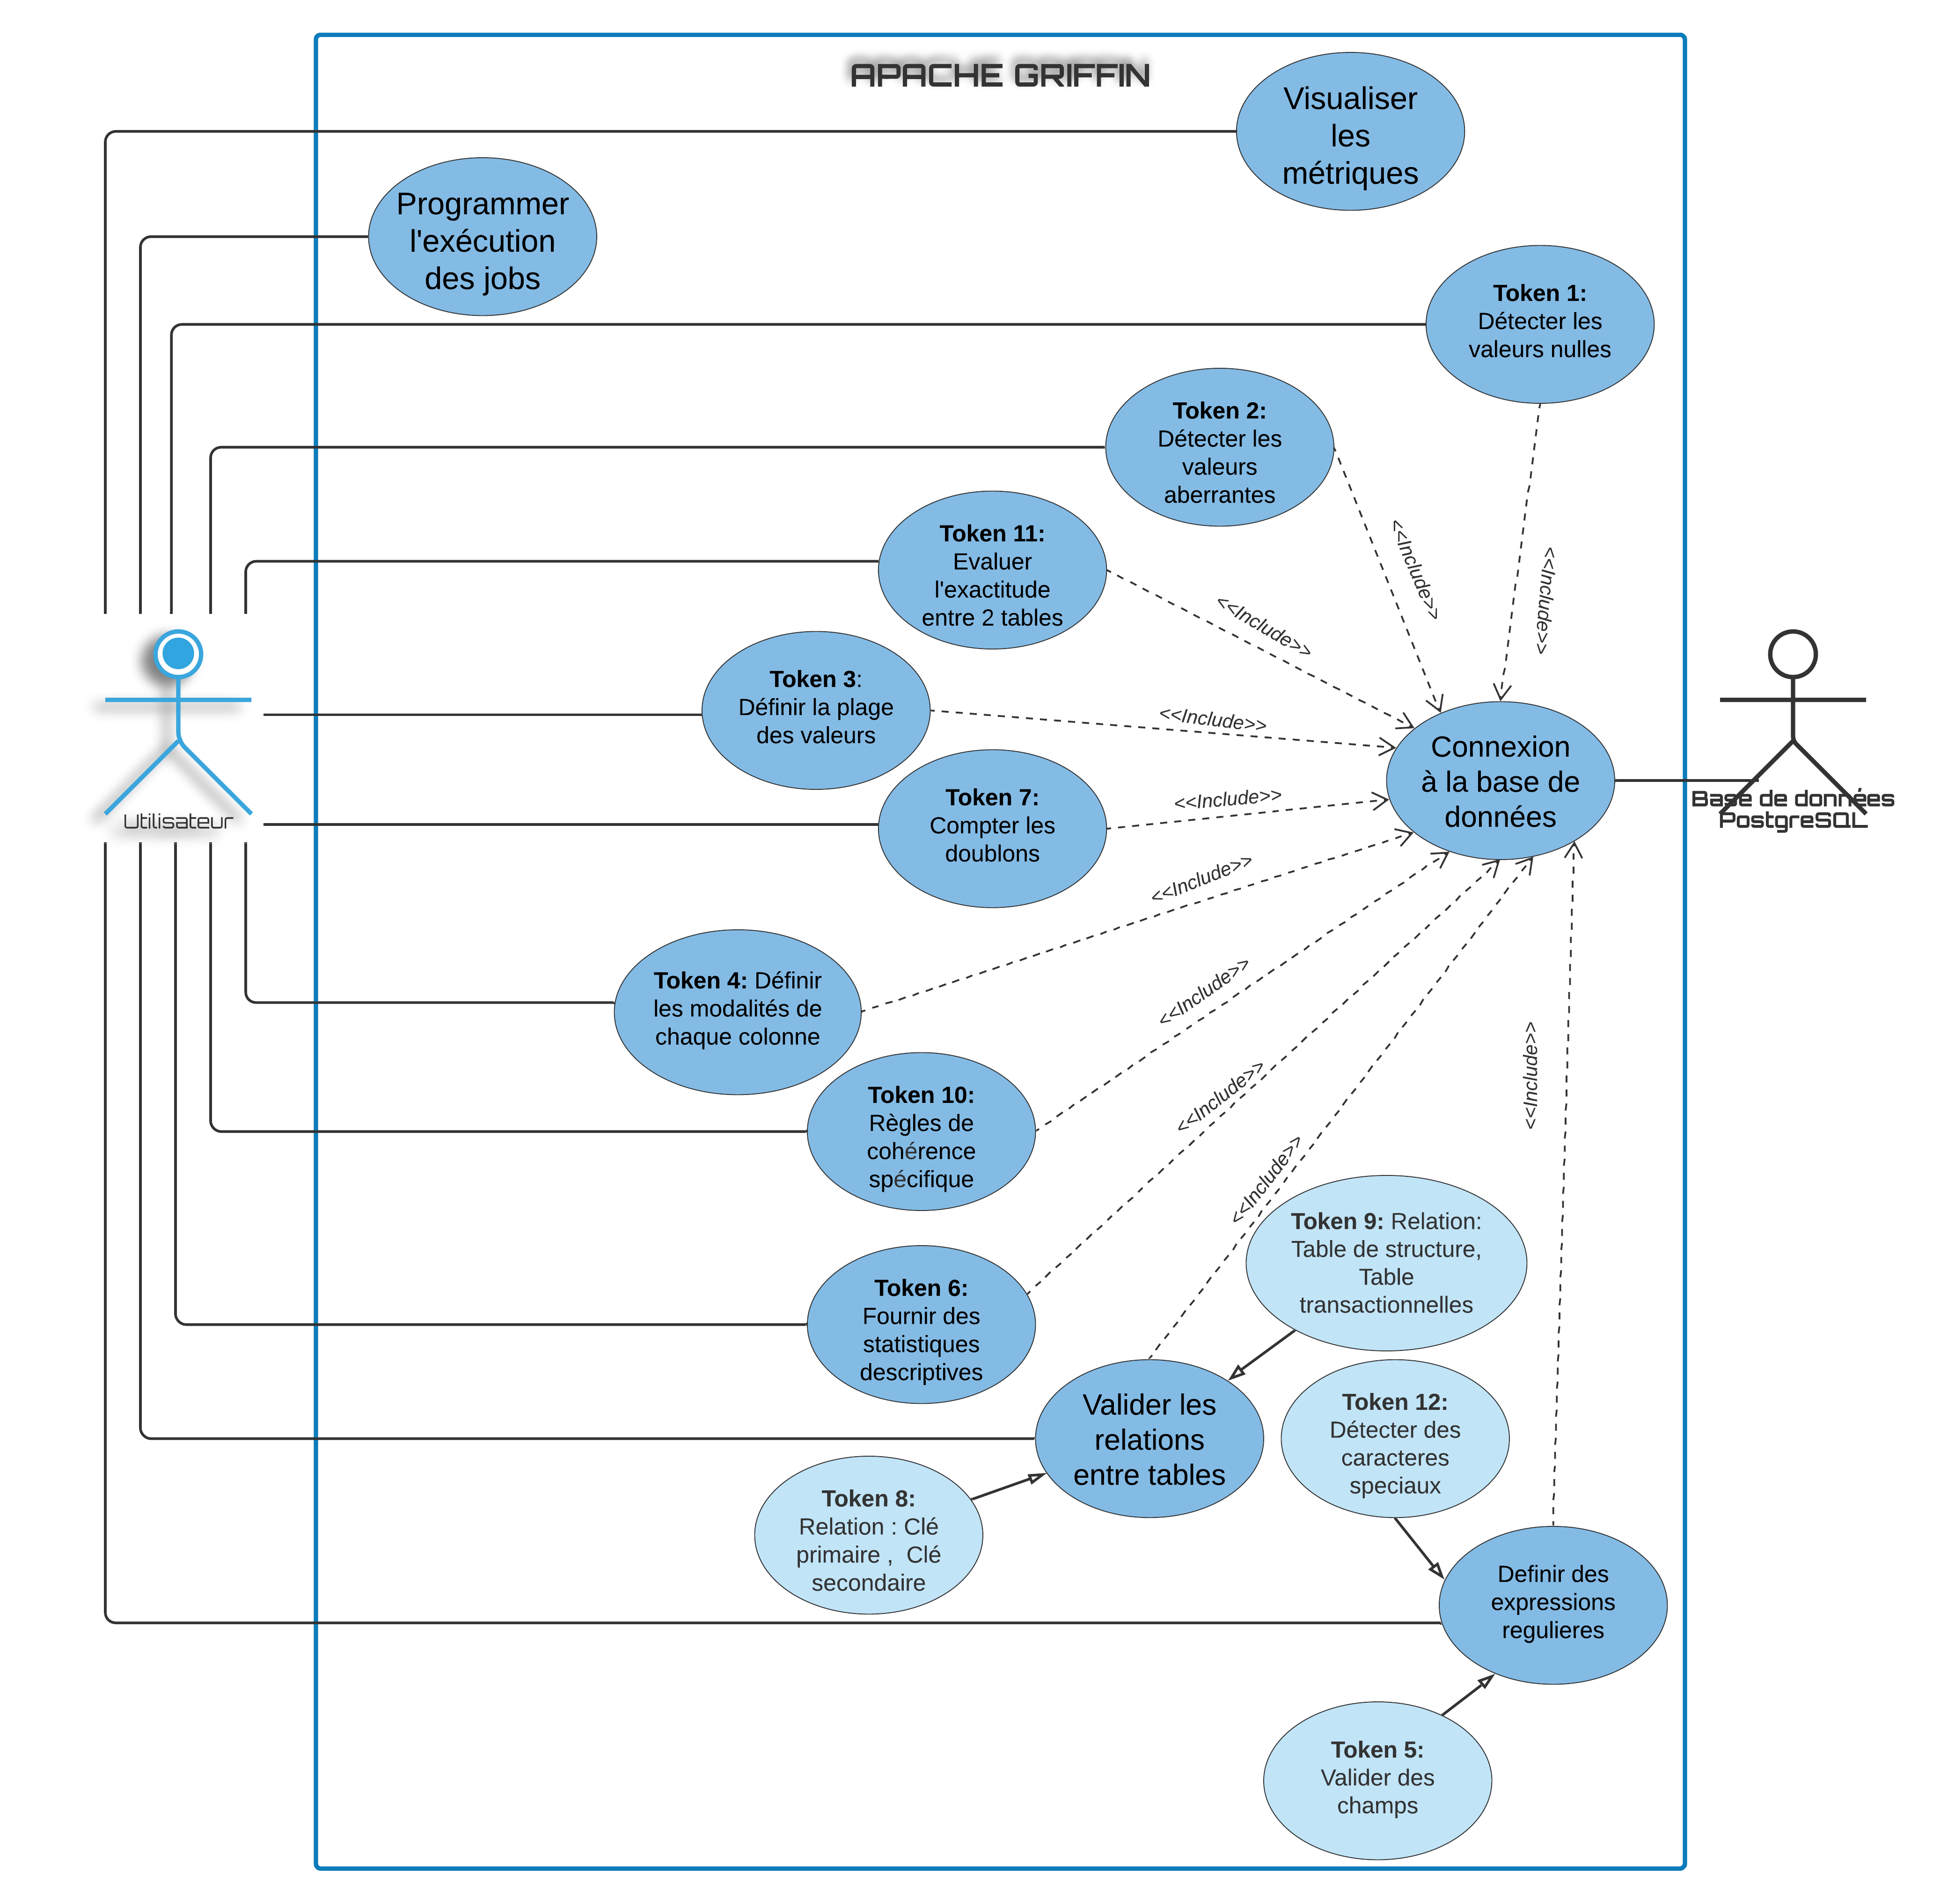
\includegraphics[scale = 0.12]{Static/Use case diagram_Griffin.png} 
    \end{center}
\end{figure}
%\end{adjustwidth}
\begin{Token}[leftmargin=2cm,parsep=0cm,itemsep=0cm]
\item  D\'etecter les valeurs nulles;  
\item  D\'etecter les valeurs aberrantes; 
\item  Définir la plage des valeurs;
\item  Définir les modalités de chaque colonne;
\item  Définir des expressions régulières pour certaines colonnes (mail, tél, Cin, Date..);
\item  Fournir des statistiques descriptives (min, max, …);
\item  Compter les doublons;
\item  Valider les \'eventuelles relations entre les tables (clé primaire, clé étrangère, …);
\item  V\'erifier que les codes des valeurs de structures sur les tables transactionnelles existent au niveau des tables de structure;
\item  Implémenter des règles de qualité (Ex : somme des primes par garantie = prime nette totale);
\item  \'Evaluer l'exactitude entre 2 tables;
\item  D\'etecter les caractères spéciaux.
\end{Token}
Nous avons eu recours \`a des donn\'ees test, afin de pouvoir \'elaborer et ajuster les diff\'erentes r\`egles permettant de valider ces tokens. Les m\'etriques obtenues, ont pu \^etre visualiser sur Kibana. Une pr\'esentation plus détaillée des r\`egles et du tableau de bord \'elabor\'e sera faite dans le chapitre suivant.\\

Afin de pouvoir programmer les jobs, \'etant donn\'e que la connexion \acrshort{jdbc} n'est pas prise en charge par l'interface graphique, nous avons utilisé Apache Airflow (version 2.1.4) pour pouvoir ordonnancer nos jobs. Apache Airflow est une plateforme de planification de flux de travail open-source, très utilisée dans le domaine de l’ingénierie des données. L'installation a \'et\'e faite via docker. \'Etant d\'ej\`a utilis\'e \`a la \acrshort{df} on pourra aisément le mettre dans les diff\'erents flux de traitement pour faciliter la mise en production. \\

Avec la pr\'esence d'un orchestrateur de t\^ache, on vient de mettre en place ainsi un syst\`eme quasi temps r\'eel. En effet, avec Apache Airflow on peut programmer l'exécution des jobs \`a une date et fr\'equence donn\'ee. La connexion \`a la base de donn\'ees est automatiquement r\'ealis\'ee \`a l'exécution d'un des cas d'utilisation (token) pr\'esent\'e plus haut. Une fois l'exécution faite, les m\'etriques et r\'esultats issus sont mis sur Elasticsearch. Le couple Elasticsearch, Kibana forme un syst\`eme pseudo temps r\'eel ainsi la visualisation des m\'etriques s'actualise automatiquement sans aucune intervention humaine. Il ne reste plus qu'\`a identifier les non-qualit\'es pour y appliquer des correctifs.


